%% This is a dissertation template for use with Masters/PhD dissertations at the University of Arizona.
%%
%% This template was created in 2022 and subsequently updated by Samuel A. Myers to greatly simplify the 
%% old thesis template. This was done to make the template easier to use, less intimidating, and because
%% the old template had not been actively updated in over a decade. Furthermore, in recent years the Grad 
%% College has greatly relaxed thesis requirmenets, and so the hyperspecific formatting guidelines utilized in
%% the old template were no longer relevant. 
%%
%% Also note that all of the AAS compatability has been explicitly removed, however it can easily be added back
%% by simply including the relevant packages in the preamble. This shouldn't break the template (with the exeption
%% of deluxetable, which is evil and should never be used).
%%
%% This template was made to match the guidelines as listed here (https://arizona.app.box.com/v/grad-gsas-dissformat)
%% in Jan of 2024. As always, check to make sure that your thesis is compliant before submitting it. If you
%% find any errors, please let the current LPL template manager or grad webmaster know. Furthermore, Be aware that 
%% there are some "secret" requirements that they don't tell you about until you are submitting your thesis. For
%% the most part these should be small things, but if you have problems, reach out to the template manager.
%%
%% This template is based on an old template that utilized a custom LaTeX class. That template was
%% worked on from the late 80's to early 2000's by a series of graduate students in the Department of
%% Planetary Sciences. Although much of that template has been scrapped, this template is still heavily based
%% on it, and much of their sample text has been utilized. The following is a list of all the students who
%% have worked on various thesis templates.
%%
%% Peter Halverson	1989 (non-LPL)
%% William D. Sears	1994
%% Rov Vervack		1996
%% Andrew Rivkin	1997
%% Joe Spitale		2001
%% Dave O'Brien		2003
%% Ross A. Beyer	2004
%% Jim Richardson	2005
%% Terry Hurford	2005
%% Curtis S. Cooper	2007
%% David A. Minton  2009
%% Samuel A. Myers	2024
%%
%% To compile this template, the recommend run sequence is:
%% PdfLaTeX + Bib(la)tex + PdfLaTeX (x2)
%% This should ensure the references, figures, tables, table of contents, etc are all updated fully and correctly.
%% If using Overleaf, Overleaf should take care of this automatically.
%%
%% If you have any questions and its before ~2026, please feel free to email sammyers@arizona.edu


\documentclass[12pt]{report} %Sets default font size and report format
    %To align the page numbers for double sided printing use \textbf{\documentclass[12pt,twoside]{report}}
    %You will also have to change a line (noted below) under Set up for fancyhdr and comment out a line
    %under both the List of Figures and List of Tables (also noted below).
    %Note that twosided page numbers are nicer for printing, but ARE NOT COMPLIANT with the requirements

%------------------------------------Import our packages----------------------------------------------
%These are all the packages required for the base template. Note that you may find other packages useful
%to deal with the particular needs for your dissertation.

\usepackage[margin=1in]{geometry}	
	%Sets 1in margin on all sides. Required for ProQuest/UMI. Note there are otherwise no margin
	%formatting requirements from the college.
\usepackage{amsfonts,amsmath,amssymb,wasysym}	
	%Includes basic math symbols, including astronomy symbols. Note some symbols may require being
	%placed in their own brakcets to work properly, ie {\odot}
\usepackage{fancyhdr} 							
	%Provides more customization of the headers
\usepackage[explicit]{titlesec}	
	%Allows for cusotmization of section heading appearances						
\usepackage{indentfirst}						
	%By default indents the first line of a paragraph
\usepackage[round]{natbib}						
	%Incredibly useful for citations. The round option puts citations in round instead of square
	%brackets. You can replace this with other packages as you see fit. May require tweaking to
	%get REFERENCES to appear in ToC
\usepackage{graphicx}
	%Package for figure inclusion
\usepackage{caption}
	%Package for manipulating figure captions
\usepackage{hyperref}
	%Governs how hyperlinks are displayed and used
\usepackage{setspace}
	%Allows manipulation of line spacing
\usepackage[titles]{tocloft}
	%Allows manipulation of the table of contents. The titles options ensures changes only apply to the
	%ToC and not the actual title formating in the main document
\usepackage{pdfpages} 
	%Allows inclusion of existing pdfs
\usepackage{bibentry}
	%Allows citing a full reference inline
\usepackage[all]{nowidow}
    %Removes "widow" and "orphan" lines, i.e. single lines at the top or bottom of a page that start
    %or end a paragraph. Some consider this one of the "secret" formatting requirements.

%--------------------------------------Set up options--------------------------------------------------

%Puts the page number in the upper right hand corner. Note a page number is required on every page except
%the title page and the title page is considered page 1. The location of the page number being in the upper
%right is one of the "secret" requirements. Note if you import other documents or rotate pages you will have
%to ensure correct placement of the page numbers.
\pagestyle{fancy} 
\fancyhead{} %Clears the default header
\renewcommand{\headrulewidth}{0pt} %Removes header rule line
\fancyhead[R]{\thepage} %Places the page number. For twosided option comment out this line
%\fancyhead[LE,RO]{\thepage} %For twosided option uncomment this line
\fancyfoot{} %Clears the default footer


%General text formatting
\setlength{\parindent}{1em} %Sets indent length
\setlength{\parskip}{0em} %Sets spacing between paragraphs
\renewcommand{\baselinestretch}{1.5} %Sets line spacing to 1.5
	%Note there are no requirements from the Grad College on these formatting choices
	%They have been set here for readability.


%Link formatting 
\hypersetup{ %Sets color of web and internal links. Can change all to black if you don't want them noticable
    colorlinks=true,
    linkcolor=blue,
    filecolor=magenta,      
    urlcolor=blue,
    pdftitle={UA Dissertation Template}, %Sets the internal file name read by programs like Chrome/Adobe
    pdfpagemode=FullScreen,
    citecolor=blue
}
\urlstyle{same}


%Figure Formatting
%\graphicspath{{"/Users/Wilbur Wildcat/My Figures/"}} %Optional path for where figures are stored
\captionsetup[figure]{labelfont={bf},font=small} %Sets label formatting and font size for figure captions
\captionsetup[table]{labelfont={bf},font=small} %Same as above for table captions


%Chapter/section appearance formating for both numbered and unnumbered chapters, sections, and subsections
\titleformat{\chapter}{\centering\bfseries}{}{0em}{\chaptertitlename{} \thechapter}[\vspace*{1.5ex}#1]
\titleformat{name=\chapter,numberless}{\centering\bfseries}{}{0em}{#1}
\titleformat{\section}{\bfseries}{}{0em}{\thesection\hspace{1em}#1}
\titleformat{name=\section,numberless}{\bfseries}{}{0em}{#1}
\titleformat{\subsection}{\itshape}{}{0em}{\thesubsection\hspace{1em}#1}
\titleformat{name=\subsection,numberless}{\itshape}{}{0em}{#1}


%Table of contents formatting
\renewcommand*\contentsname{TABLE OF CONTENTS} %Renames table of contents
\renewcommand\cftchapdotsep{\cftdotsep} %Inserts dot leader for chapters
\renewcommand{\cftsecfont}{\bfseries} %Bold section titles
\renewcommand{\cftsubsecfont}{\itshape} %Italicize subsection titles
\renewcommand{\cftchappagefont}{\normalfont} %Removes bolding from chapter page numbers
\renewcommand{\cftchapleader}{\normalfont\cftdotfill{\cftsecdotsep}} %Removes bolding for chapter dot leader
\renewcommand\cftchappresnum{\MakeUppercase\chaptername{} } %Prints CHAPTER in front of each chapter
\addtolength\cftchapnumwidth{6em} %Affects spacing between CHAPTER and the chapter name

%Same as above two commands except for appendices
\makeatletter
\g@addto@macro\appendix{
  \addtocontents{toc}{
    \protect\renewcommand{\protect\cftchappresnum}{\MakeUppercase\appendixname{} }
    \addtolength\cftchapnumwidth{1em}
  }
}
\makeatother

%Renames figure and table list
\renewcommand{\listfigurename}{LIST OF FIGURES}
\renewcommand{\listtablename}{LIST OF TABLES}


%Bibliography formatting
\bibliographystyle{abbrvnat} 
	%Sets citation style. Can be replaced as desired. Note that the Grad College does not require a specific
	%format.
\newcommand*{\doi}[1]{\href{http://dx.doi.org/#1}{doi: #1}}
    %Automatically turns any DOIs in the references into hyperlinks
\renewcommand{\bibsection}{} %Hides default References title



%---------------------------------------------Custom Values-------------------------------------------------
% These are custom values mainly (exclusively) used to make the title page. Change them as necessary
\newcommand{\CompleteTitle}{How to Construct a Template for a UA Thesis} %The complete title of your dissertation
\newcommand{\FullName}{Gerard Peter Kuiper} %Your full name
\newcommand{\DegreeType}{Doctor of Philosophy} %Your type of degree
\newcommand{\DepartmentName}{Department of Planetary Sciences} %Your department name
\newcommand{\DegreeYear}{2024} %Year of your degree



\begin{document}	%Start the document
\nobibliography* %This is necessary for bibentry to work correctly. If not using bibentry you can comment it out


%---------------------------------------------Title Page--------------------------------------------------
% This page must be formatted as shown here, unless your major does not match the name of your department.
% In this case please refer to the Grad College guidelines. 

\thispagestyle{empty} %Removes page number

\null
\vfill
	%Sets vertical spacing

\begin{center}
\MakeUppercase\CompleteTitle \\ 
\vspace*{1.5em}
by\\
\vspace*{1.5em}
\FullName \\
\vspace*{2em}

\rule{3in}{1pt}\\
\vspace*{-1em}
{\small Copyright \copyright\ \FullName\ \DegreeYear} \\
\vspace*{2em}

A Dissertation Submitted to the Faculty of the\\
\vspace*{1.5em}
\MakeUppercase\DepartmentName \\
\vspace*{1.5em}
In Partial Fulfillment of the Requirements\\
\vspace*{0.5em}
For the Degree of\\
\vspace*{1.5em}
\MakeUppercase\DegreeType \\
\vspace*{1.5em}
In the Graduate College\\
\vspace*{1.5em}
THE UNIVERSITY OF ARIZONA\\
\vspace*{3em}
\DegreeYear
\end{center}

\vfill %Needed for vertical spacing





% ----------------------------------------Approval Page-------------------------------------------------
% Copy the form you need from https://grad.arizona.edu/gsas/dissertations-theses/sample-pages.
% Edit the form in Word as appropriate and save as a pdf. Have your form physically or electronically 
% signed and save it as a pdf. Include it using the following command.

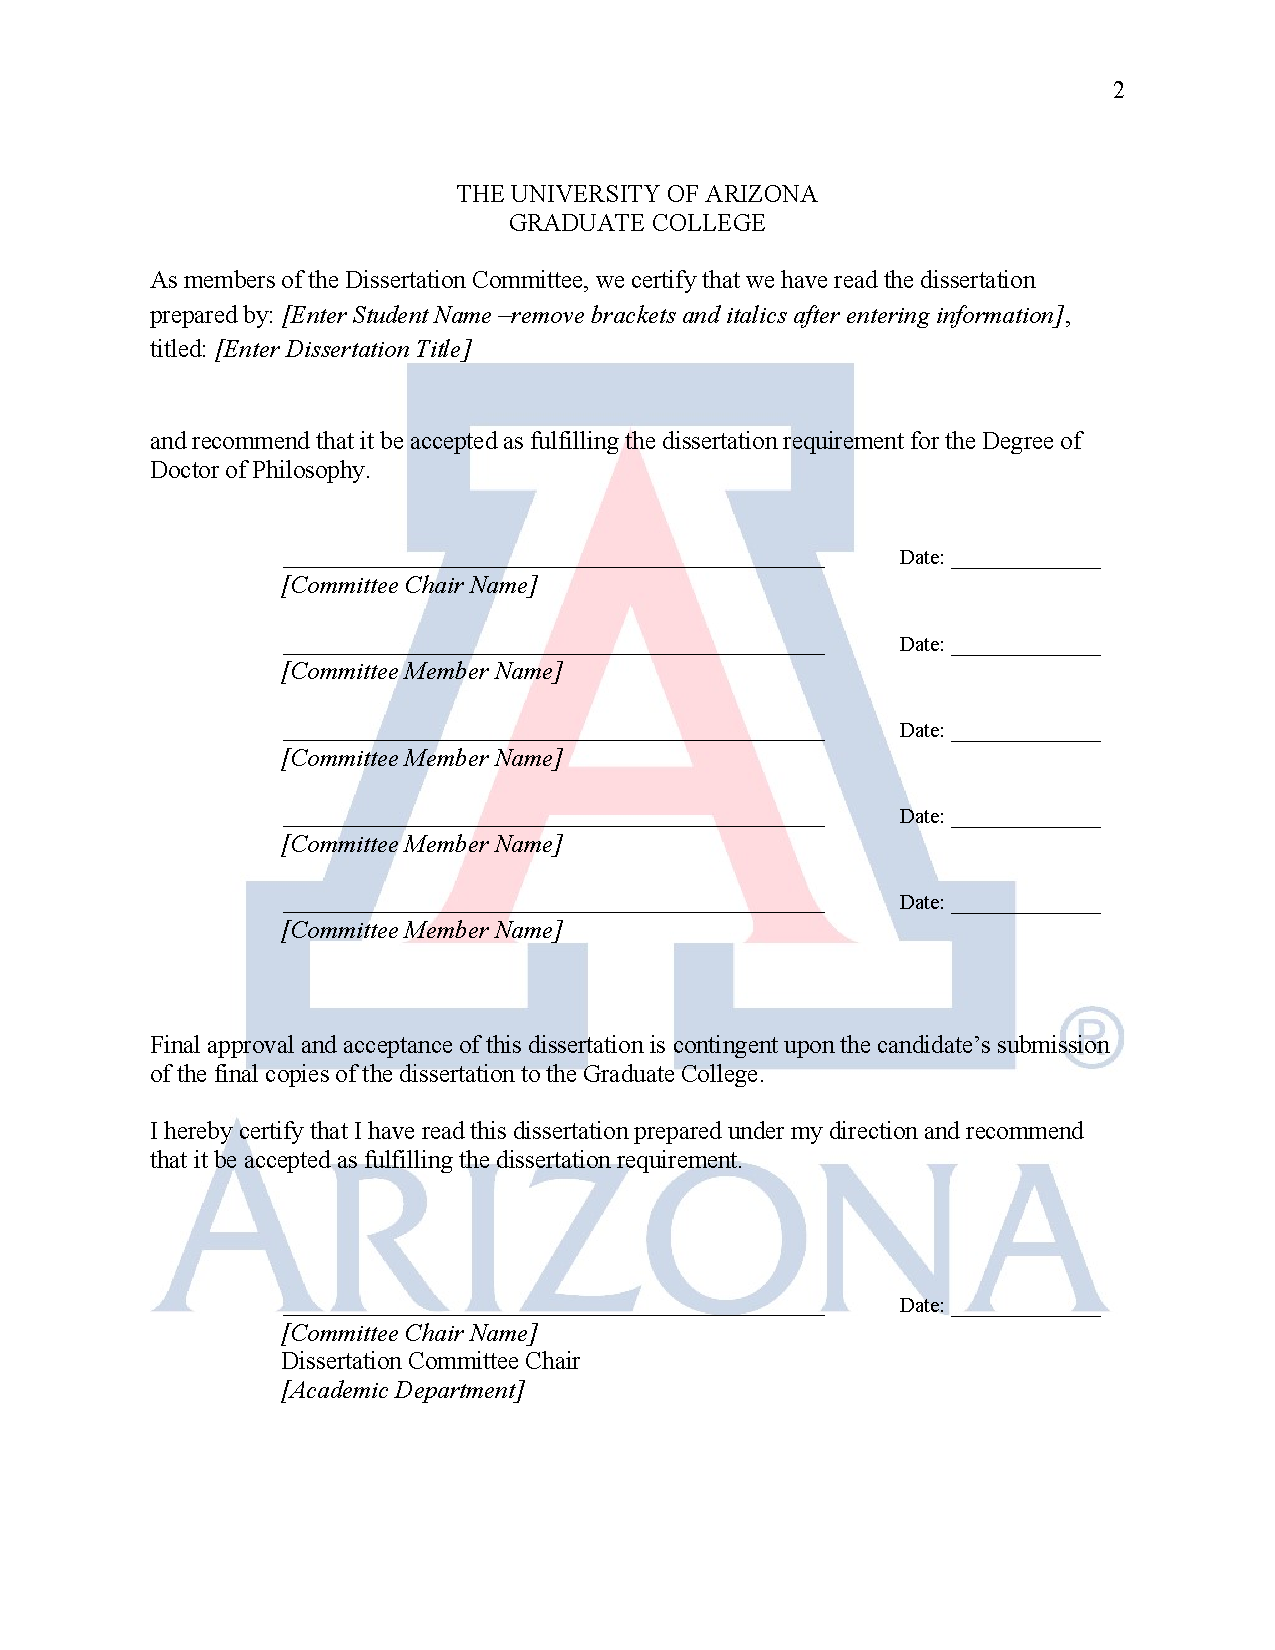
\includepdf[pages={1}]{signed_approval_page.pdf} % Name of signed approval form, in pdf format





%---------------------------------------Acknowledgments------------------------------------------------
% This section is optional. To remove it simply comment out all of the lines betweeen here and the next
% section.
\chapter*{ACKNOWLEDGMENTS}
\thispagestyle{fancy} %Resets custom page number location and first chapter page

Insert your acknowledgments here. They will have the same formatting as the rest of the document. They
should be limited to one page, although this is not explicitly listed in the formatting requirements.





%---------------------------------------Land Acknowledgment------------------------------------------------
% This section is optional. To remove it simply comment out all of the lines betweeen here and the next
% section. Note if you do include it, you cannot change any of the wording. If you want to change the wordng
% some students have been allowed to change the title of the chapter to "PERSONAL STATEMENT ON LAND
% ACKNOWLEDGEMENT".
\chapter*{LAND ACKNOWLEDGMENT}
\thispagestyle{fancy} %Resets custom page number location and first chapter page

\noindent We respectfully acknowledge the University of Arizona is on the land and territories of Indigenous peoples.
Today, Arizona is home to 22 federally recognized tribes, with Tucson being home to the O'odham and the Yaqui.
Committed to diversity and inclusion, the University strives to build sustainable relationships with sovereign
Native Nations and Indigenous communities through education offerings, partnerships, and community service.





%----------------------------------------------Dedication------------------------------------------------
% This section is optional. To remove it simply comment out all of the lines betweeen here and the next
% section. This should be limited to one page, although this is not explicitly listed in the formatting
% requirements.
\chapter*{DEDICATION}
\thispagestyle{fancy} %Resets custom page number location and first chapter page

\begin{center}
\textit{Dedicated to Bratfest and how it allowed me to numb the pain.}
\end{center}





%--------------------------------------Table of Contents--------------------------------------------------
% Note that at all entries in the TOC must be formatted as they are in the text, i.e. if a title is bolded
% in the text it must be bolded in the TOC. This will be done automatically if you don't change any of the
% formating.
\tableofcontents
\thispagestyle{fancy} %Resets custom page number location





%----------------------------------------List of Figures--------------------------------------------------
%Technically optional but highly encouraged if you have any figures.
\cleardoublepage %Ensures accurate page numbering. If using the twosided option comment out this line
\phantomsection %Needed for hyperref
\addcontentsline{toc}{chapter}{\listfigurename} %Includes figure list in table of contents
\listoffigures
\thispagestyle{fancy} %Resets custom page number location





%----------------------------------------List of Tables--------------------------------------------------
%Technically optional but highly encouraged if you have any figures.
\cleardoublepage %Ensures accurate page numbering. If using the twosided option comment out this line
\phantomsection %Needed for hyperref
\addcontentsline{toc}{chapter}{\listtablename} %Includes table list in table of contents
\listoftables
\thispagestyle{fancy} %Resets custom page number location





%------------------------------------------------Abstract--------------------------------------------------
\chapter*{ABSTRACT}
\thispagestyle{fancy} %Resets custom page number location on page
\addcontentsline{toc}{chapter}{ABSTRACT}

This is where the body of your abstract goes. The abstract should summarize your work. There is no formal 
length limit/requirement that I could find as of the creation of this template.





%----------------------------------------Example Chapter--------------------------------------------------
\chapter{Sample Chapter}
\thispagestyle{fancy} %Resets custom page number location on first chapter page

\section{Introduction}
This is an example of a numbered section. You can also created unnumbered sections and subsections, although
I recommend against it. If you create unnumbered sections you will have to add them to the Table of Contents 
manually with the \texttt{addcontentsline} command. \footnote{By the way footnotes are a thing}.\\

\textit{Note: All titles (chapters, sections, subsections, etc. must be in Title Case.)} 

\section*{An Unnumbered Section}
This is an unnumbered section that has not been added to the Table of Contents.

\subsection{Subsections!}
You can also create subsections. They follow the same rules as sections.


\section{Math Example}
This is a real short example of using the equation environment.

\begin{equation}
	y = mx + b
\end{equation}

There is an awful lot that the equation environment and math mode can do for you.


\section{References}
Here is an example of references using the natbib package. You can reference in a number of ways.  The
ones that are most useful are parenthetical \citep{article,articletwo} or inline, as in \citet{articletwo} 
said this or that. You can also include information within the citation \citep[e.g.][doesn't have any
page numbers]{2003jgr}.  You don't even need to have the reference in your text to be included (see .tex file). 
\nocite{2004LPI}

You can also cite your references directly inline using the \texttt{bibentry} command as follows: \bibentry{article}


\section{Figures} \label{section:figures}
On the next page is a figure inclusion using the `graphicx' package. This puts figures on their own page by 
themselves. They don't need to be on separate pages, there is no requirement that they be on separate pages.
If you want to put a figure on a page with text, don't include the \emph{p!} option in square brackets at 
the begin figure command.

You can use most common file types with this package. Just make sure the file extension listed in the command
matches the actual file.

Also note that the \verb=\caption= command has an optional square-bracketed argument and a curly-bracketed 
argument.  Whatever you put in square brackets will be used as the short caption, and will go into the 
List of Figures.  The stuff in the curly brackets will be placed on the page under your figure.


\begin{figure}[p!]
\begin{center}
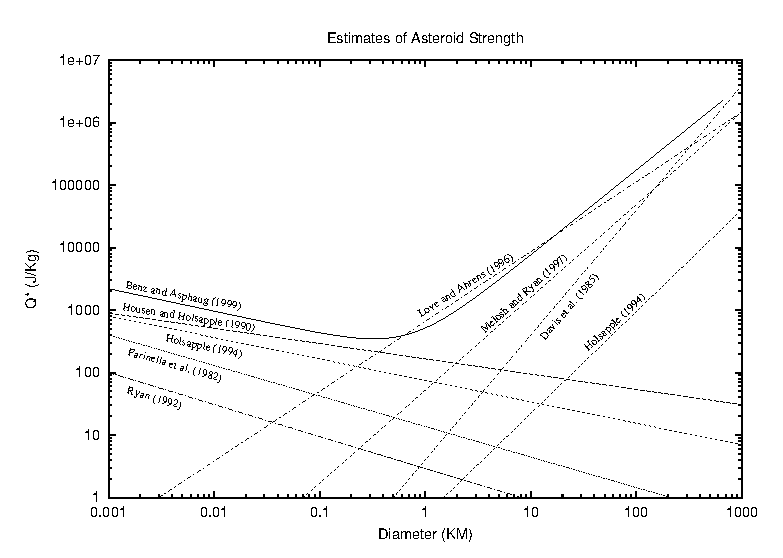
\includegraphics{figure.eps}
\caption[Short figure caption for LOF]{Sample figure caption (to appear below
the actual figure). \label{samplefig}}
\end{center}
\end{figure}

You can reference a figure later using the \verb=\label= command (Figure~\ref{samplefig}). This can also be
done for sections and chapters (Section~\ref{section:figures}).





%----------------------------------Example Chapter 2: Electric Boogaloo-----------------------------------------
% You can also use the input command to include separate tex files. Try to avoid the input command as it may 
% break the formatting (or more often just straight up not work).
\chapter{Another Example} 
\thispagestyle{fancy} %Resets custom page number location on first chapter page

\section{Big Files}
For big projects (like a thesis) it is sometimes helpful to separate your chapters indo different documents. This
can be done with the \verb=\input= command. Simply save your chapter as a separate .tex file without a header or
preamble, and then input it into the main dissertation file. Try to avoid using the \verb=\include= command as \LaTeX\
can get cranky with the formatting when ``including'' a .tex file.

\section{Non-Breaking Spaces}
The tilde character can be used to mark a non-breaking space. \LaTeX\ does a great job of lining words up, putting
in line breaks where appropriate, and making the text flow properly. However, there are some cases where you really
don't want \LaTeX\ to toss in a carriage return. The places that spring to mind are between numbers and their units,
and between Figure and Table references and their values. So for example, you don't want something like this in your
document:

\begin{quote}
	Blah blah blah blah blah blah blah blah blah is 10\\
	m from foo to bar.
\end{quote}

So always use the tilde when you use numbers with units, like 9.8~m~s$^{-2}$, and with references, like Figure~\ref{samplefig}.
This way \LaTeX\ will never put a line break between those elements.


\section{Hyperlinks}
You may have noticed a lot of blue text in this template. Those are internal hyperlinks that are automatically set up by 
the \texttt{hyperref} package. You can change the colors of the links by messing with the options in the preamble. For the
most part these links should set themselves up to work just fine by themselves. If you notice weird behavior you can usually
find solutions online. If not the use of the hyperlinks is purely for convenience when working with large documents and is not
required by the Grad College.

You can also use this package to include web links. Long links can sometimes escape the page margins though, so I recommend
giving them custom text: \href{https://grad.arizona.edu/gsas/dissertations-theses/dissertation-and-thesis-formatting-guides}
{A link to the UA Thesis guidelines.}

\section{Tables}
On the next page is a sample table, placed on the page by itself. Again, this table is pretty small, so it could 
probably just be placed on a page with text. To do this remove the \emph{p!} from the command. Working with tables in
\LaTeX\ is notoriously difficult (although Overleaf has made it easier of late), so make liberal use of StackExchange 
and Google. 

A comment on \texttt{deluxetable}. \texttt{deluxetable} is a special table package from the AAS formatting standards that
some people insist is much nicer than the default \LaTeX\ table. These people are wrong, and \texttt{deluxetable} is evil.
Therefore I have not included a way for this template to work with \texttt{deluxetable}. If you want to try, that's your
choice, but I cannot guarantee it won't break the template.

\begin{table}[p!]
\begin{center}
\caption[Short table caption for LOT]{Sample table caption (to appear with the actual table). \label{sampletable}}
\vspace{0.3in}
\begin{tabular}{ccc}
\hline 
\hline
Col A & Col B & Col C \\
\hline
1 & 2 & 3 \\
4 & 5 & 6\\
\hline
\end{tabular}
\end{center}
\end{table}

By the way, you can reference Tables like you can figures (Table~\ref{sampletable}).





%----------------------------------------Appendices--------------------------------------------------------
% Appendices are not required. To remove them simply comment out all of the lines betweeen here and the next
% section. There is no limit on the number of appendices. If included they must go after regular chapters and
% before the references.
\appendix
\chapter{A Wild Appendix Appeared}
\thispagestyle{fancy} %Resets custom page number location on first appendix page

This is an appendix. Put appendixy things in it.





%----------------------------------------References--------------------------------------------------
\chapter*{References}
\thispagestyle{fancy} %Resets custom page number location and first references page
\addcontentsline{toc}{chapter}{REFERENCES} %Includes references in table of contents
\bibliography{bibliography} %Natbib reference list. Value in brackets should be name of .bib file


\end{document}